\documentclass[a4paper,11pt]{article} 

\usepackage[spanish]{babel}
\usepackage[utf8]{inputenc}

\usepackage{geometry, amsmath, amssymb}
\geometry{margin=2.5cm}

\usepackage{hyperref}
\usepackage{microtype} 

\usepackage{fancyhdr}
\usepackage{graphicx}

% me parece que con esto manejo los colores
\usepackage{color, soul}

\pagestyle{fancy}
\fancyhf{}
\lhead{Guía de Ejercicios 4}
\rhead{Tecnología Digital VI}
\cfoot{\thepage}

\title{\vspace{-2cm}\textbf{Guía de Ejercicios 4}\\[0.2cm]
\large Tecnología Digital VI}
\author{Juan Ignacio Elosegui}
\date{Universidad Torcuato Di Tella \\ Junio 2026}

\begin{document}
\maketitle

\section*{Introducción a redes neuronales y arquitectura}
\subsection*{Ejercicio 1}
El operador XOR no puede ser aprendido por un perceptrón original porque la función de los valores de X e Y como entradas no pueden ser separados linealmente, por lo que con una sola neurona no se puede hacer.

Con dos neuronas, se introduce una no linealidad capaz de separar el gráfico de manera apropiada.
\subsection*{Ejercicio 2}
Un MLP tiene más capas y más neuronas que un perceptrón simple. Al tener más capas \textit{fully-connected}, se implementa la no linealidad que aporta un plus a lo que es la capacidad de aprendizaje.

\section*{Funciones de activación}
\subsection*{Ejercicio 3}
La no linealidad es importante porque (1) los datos en el mundo real no suelen ser linealmente separables, (2) permite a la red neuronal que cree barreras de decisión curvas para poder manejar patrones complejos en los datos, y (3) se aseguran que las redes puedan modelar problemas complejos como es el reconocimiento de imágenes.

Si una red neuronal tuviese únicamente funciones de activación lineales, lo que se dará es que la última capa será una combinación lineal de todos los inputs anteriores. Esta red será incapaz de aprender patrones interesantes más allá de los lineales.
\subsection*{Ejercicio 4}
Cuando se entrena una red neuronal, se usa un algoritmo llamado \textit{backpropagation} para calcular cuánto deberían cambiar los pesos de cada neurona para minimizar el error general del modelo. Los ajustes a estos pesos dependen del gradiente de la función de pérdida (error), que esencialmente mide cómo cambia el error a medida que se ajustan los pesos. Pero en redes profundas con muchas capas, estos gradientes pueden volverse muy pequeños (es decir, se ``desvancen'') en ciertas capas, especialmente aquellas lejos de la capa de salida.

Cuando el gradiente se aproxima a cero, los pesos dejan de actualizarse, deteniendo efectivamente el proceso de aprendizaje en esas capas. Este es el problema \textbf{vanishing gradient}, que ralentiza o incluso impide que la red neuronal mejore durante el entrenamiento.

Este problema es común en funciones de activación como la sigmoide o Tanh, porque mapean valores grandes de input a un rango pequeño de output. Como resultado, cuando se calculan los gradientes, tienden a volverse muy chicos, en especial cuando se multiplican a través de muchas capas durante backpropagation.
\subsection*{Ejercicio 5}
Las neuronas con ReLU tienen output cero y derivada cero cuando sus inputs son negativos. Entonces, si los pesos en la red siempre tienden a pasarle un número negativo a una neurona ReLU, esa neurona no va a contribuir al entrenamiento de la red, porque su contribución a las actualizaciones de los pesos que vengan de esa neurona siempre serán cero.

Para solucionar este problema, se pueden usar variaciones de ReLU (Leaky ReLU, PReLU, ELU...) cuya forma permite generar pequeños outputs negativos cuando su input es cero. Esto quiere decir que no hay segmentos de la función que tengan derivada igual a cero.
\subsection*{Ejercicio 6}
Para cualquier vector \(z = [z_{1}, z_{2}, \ldots, z_{n}]\), la función Softmax se define como: $$\sigma(z_{i}) = \frac{\exp(z_{i})}{\sum_{j=1}^{n}\exp(z_j)}$$ donde \(\exp(z_{j})\) es la exponenciación del valor de input, y \(\sum_{j=1}^{n}\exp(z_j)\) es la suma de todos los valores exponenciados para normalizar los outputs. Cada output de \(\sigma(z_{i})\) representa la probabilidad de la clase $i$.

La normalización es clave para que convierta los logits en una distribución probabilística donde la suma de todos ellos dé como resultado 1.

\section*{Forward y backward propagation}
\subsection*{Ejercicio 7}
\textbf{Forward propagation} es el proceso en el cual los datos de input pasan a través de las capas de la red para producir un output. Transforma inputs en predicciones usando pesos, biases y funciones de activación. Preferentemente, el input debe ser normalizado o estandarizado antes de ser procesado por las capas.

\textbf{Backward propagation} es el proceso en el cual se entrena a las redes neuronales para que bajen su error de predicción. Funciona propagando los errores hacia atrás, calculando gradientes usando la regla de la cadena y actualizando los pesos y biases para mejorar el rendimiento.
\subsection*{Ejercicio 8}
\begin{figure}[h]
    \centering
    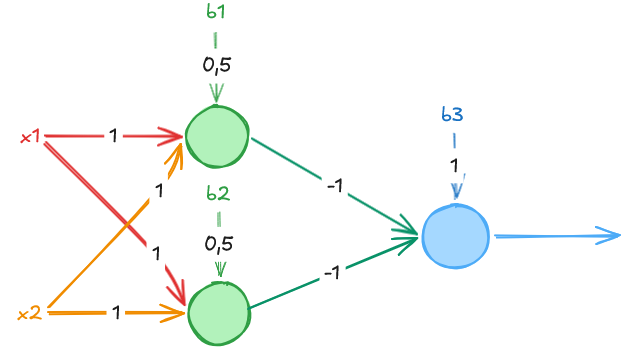
\includegraphics[width=0.6\textwidth]{img/1.png}
\end{figure}

\subsection*{Ejercicio 9}
\hl{Pedirle a Chino}
\subsection*{Ejercicio 10}
Los \textbf{grafos computacionales} son una manera de representar expresiones matemáticas, donde cada hoja representa una variable y cada nodo intermedio representa una operación.

Para representar la función \(f(x, y, z) = (x+y) \times z\), se puede usar el grafo:
\begin{figure}[h]
    \centering
    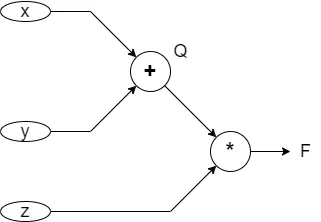
\includegraphics[width=0.4\textwidth]{img/2.png}
\end{figure}

Para calcular el output, se propaga el input por la red.

\hl{No entiendo el uso funcional para una red neuronal. ¿Qué se quiere conseguir al fin y al cabo?}
\section*{Optimización, hiperparámetros y regularización}
\subsection*{Ejercicio 11}
\subsection*{Ejercicio 12}
\subsection*{Ejercicio 13}
\subsection*{Ejercicio 14}
\subsection*{Ejercicio 15}

\end{document}